%% LaTeX-Beamer template for KIT design
%% by Erik Burger, Christian Hammer
%% title picture by Klaus Krogmann
%%
%% version 2.0
%%
%% mostly compatible to KIT corporate design v2.0
%% http://intranet.kit.edu/gestaltungsrichtlinien.php
%%
%% Problems, bugs and comments to
%% burger@kit.edu

\documentclass[18pt]{beamer}
\usetheme{kit}

%% TITLE PICTURE

% if a custom picture is to be used on the title page, copy it into the 'logos'
% directory, in the line below, replace 'mypicture' with the 
% filename (without extension) and uncomment the following line
% (picture proportions: 63 : 20, *.eps format if you use latex+dvips+ps2pdf,
% *.jpg/*.png/*.pdf if you use pdflatex)

%\titleimage{mypicture}

%% TITLE LOGO

% for a custom logo on the front page, copy your file into the 'logos'
% directory, insert the filename in the line below and uncomment it

%\titlelogo{mylogo}

% (*.eps format if you use latex+dvips+ps2pdf,
% *.jpg/*.png/*.pdf if you use pdflatex)

%% BIBTEX ICON/KEY

% if you want to see BibTeX keys in the references view instead of the symbol,
% uncomment the following line
% \usebibitemtemplate{\insertbiblabel}

% the presentation starts here

% change the following line to "ngerman" for German style date and logos
% change the following line to "english" for English style date and logos
\selectlanguage{ngerman}

\beamertemplatenavigationsymbolsempty

\usepackage{listings}
\definecolor{darkgray}{rgb}{0.95,0.95,0.95}
\definecolor{darkgreen}{rgb}{0.05,0.7,0.05}
\lstset{ language=Java,
	backgroundcolor=\color{darkgray}, 
	numbers=none, 
	keywordstyle=\color{black}\bfseries,
	tabsize=2,
	showspaces=false,               % show spaces adding particular underscores
	showstringspaces=false,         % underline spaces within strings
	showtabs=false, 
}



\title[Short title]{Tutorium 01: Projektplanung }
\subtitle{Softwaretechnik im SS 2011, Tutorien 4 + X + 17}
\author{Jürgen Walter}
\date{3. Mai 2011}  			%%%%%%%%%%%%%%%	DATUM, anpassen!

\institute{Chair for Software Design and Quality}

\begin{document}

%title page
\begin{frame}
\titlepage
\end{frame}

\section{Organisatorisches}

\subsection{Vorstellung}
\frame{
\frametitle{Wer bin ich?}
\begin{itemize}
\item Jürgen Walter
\pause
\item 8tes Semester Informatik
\pause
\item juergen.walter.halle@gmail.com
\item uxccx@student.kit.edu
\pause
\item Partnerturoren Christian Juelg und Daniel Deckers
\item \dots
\end{itemize}
}

%table of contents
\frame{
\frametitle{Was machen wir heute?}
\tableofcontents
}

\subsection{Übungsschein}
\frame{
\frametitle{Übungsschein}
\begin{block}{Der Übungsschein \dots}
\begin{itemize}
\pause
\item ist keine Vorraussetzung zur Klausur, aber Vorraussetzung für Modul!
\pause
\item hat 6 Übungsblätter mit  insgesamt 150 Punkten
\pause
\item ist mit 50 Prozent aus Übungsblättern und Programmmieraufgaben bestanden 
\end{itemize}
\end{block}
}


\section{Altes Übungsblatt und Wiederholungen}

\subsection{Altes Übungsblatt}
\frame {
\frametitle{Altes Übungsblatt}
\begin{block}{Aufgabe 1: Mailingliste}
\begin{itemize}
\item ...
\end{itemize}
\end{block}


\begin{block}{Aufgabe 2: Lastenheft}
\begin{enumerate}
\item Zielbestimmung
\item Produkteinsatz
\item Funktionale Anforderungen
\item Produktdaten
\item Nichtfunktionale Anforderungen
\item Systemmodelle
\begin{itemize}
	\item Szenarien
	\item Anwendungsfälle
\end{itemize}
\item Glossar (Begriffslexikon zur Beschreibung des Produktes)
\end{enumerate}
\end{block}
}

\frame {
\begin{block}{Aufgabe 3 Durchführbarkeitsuntersuchung} 
\begin{itemize}
\item jeden der 6 Aspekte ansprechen
\item “Probleme durch ... treten nicht auf da ...” ist auch eine gute Antwort
\end{itemize}

\end{block}
\begin{block}{Aufgabe 4 Hans Olo}
\begin{itemize}
\item \textbf{Benutzt Checkstyle!}
\end{itemize}
\end{block}

\begin{block}{Aufgabe 5 Vorbereitung der Programmieraufgabe}
\begin{itemize}
\item ...
\end{itemize}
\end{block}
}

\subsection{Zum Aufwärmen ...}
\frame {
\frametitle{Wahr oder falsch?}
\begin{itemize}
	\color<2->[rgb]{0,1,0}
	\item In der Planungsphase wird die softwaretechnische Realisierbarkeit eines Produktes untersucht
	\color[rgb]{0,0,0}
	\pause
	\color<3->[rgb]{1,0,0}
	\item Ein Pflichtenheft beschreibt die Eigenschaften, die das Produkt aus der Sicht des Kunden erfüllen soll
	\color[rgb]{0,0,0}
	\pause
	\color<4->[rgb]{0,1,0}
	\item In einem UML-Anwendungsfalldiagramm werden typische Interaktionen des Benutzers mit dem System modelliert
	\color[rgb]{0,0,0}
	\pause
	\color<5->[rgb]{1,0,0}
	\item Das Lastenheft ist eine Verfeinerung des Pflichtenheftes
	\color[rgb]{0,0,0}
	\pause
	\color<6->[rgb]{1,0,0}
	\item Im Pflichtenheft steht beschrieben, wie etwas zu implementieren ist. Es werden z.B. Algorithmen und Datenstrukturen beschrieben
	\color[rgb]{0,0,0}
\end{itemize}
}


\subsection{Werkzeuge}

\frame{
\frametitle{Versionsverwaltungen}

\begin{block}{Subversion}
\begin{itemize}
\item von der Vorlesung unterstützte Versionsverwaltung
\item Windows: Tortoise SVN
\item Linux: Shell oder RabbitVCS
\item Mac: Shell
\end{itemize}
\end{block}
}

\frame{
\frametitle{Versionsverwaltungen\dots}

\begin{block}{Git}
\begin{itemize}
\item Werkzeug des Tutors ;-)
\item dezentrales VCS: jeder Benutzer hat lokal ein vollständiges Repository
\item hat mehr Funktionen als SVN, aber auch mehr Möglichkeiten sich selbst in den Fuß zu schießen\dots
\item Verschmelzen verschiedener Zweige und Versionen ist hier eher Normalfall als Ausnahme
\end{itemize}
\end{block}
}

\frame{
\frametitle{Versionsverwaltungen\dots}

\begin{block}{weitere}
\begin{itemize}
\item Es gibt noch viele weitere frei verfügbare dezentrale VCS
\item diese unterscheiden sich wenig voneinander
\item Mercuarial / Hg, neben Git vermutlich das verbreitetste DVCS
\item Bazaar / bzr
\item Darcs
\end{itemize}
\end{block}
}

\frame {
\frametitle{Klausuraufgabe 2009}
\begin{block}{Aufgabe}
Erklären Sie die beiden Begriffe „Striktes Ausbuchen“ und „Optimistisches Ausbuchen“ im Kontext einer Konfigurationsverwaltung. Nennen Sie jeweils einen Vor- sowie einen Nachteil. (4P)
\end{block}

Striktes Ausbuchen
\visible <2-> {
\begin{itemize}
\item Nur eine Ausbuchung gleichzeitig ist erlaubt 
\item Ausbucher hat exklusives Änderungsrecht 
\item Vorteil: kein Verschmelzungsaufwand beim Zurückschreiben 
\item Nachteil: immer nur einer kann eine Version ändern
\end{itemize}
}
Optimistisches Ausbuchen 
\visible<3-> {
\begin{itemize}
\item Mehrere Ausbuchungen gleichzeitig erlaubt 
\item Mehrere Entwickler Arbeiten an der gleichen Programmversion 
\item Vorteil: Mehrere Entwickler können eine Version ändern 
\item Nachteil: Aufwand beim Zusammenführen der Versionen (der Schnellere gewinnt)
\end{itemize}
}
}


\frame{
\frametitle{Checkstyle}
\begin{alertblock}{Das geht besser \dots}
\begin{itemize}
\item Keiner von euch ist ohne Checkstyle Fehler
\end{itemize}
\end{alertblock}

\pause
\begin{block}{private Konstruktoren und utility classes}
\begin{itemize}
\item ist alles in einer Klasse \texttt{static}, dann sollte man diese Klasse vermutlich nicht instanziieren
\item durch einen privaten Konstruktor verhindert man das versehentliche Instanziieren:\\
\texttt{ private MyClass() \{\} }

\end{itemize}
\end{block}
}

\frame{
\frametitle{Checkstyle in Eclipse}

\begin{block}{Ergebnisse anzeigen}
\begin{itemize}
\item sobald Checkstyle richtig konfiguriert wurde, gibt es einige hilfreiche Übersichten
\item \texttt{Window > Show View > Other > Checkstyle}
\item hier gibt es \texttt{Checkstyle violations}, \texttt{Checkstyle violations chart} und \texttt{Duplication Code}
\end{itemize}
\end{block}
}

\frame{
\frametitle{Eclipse - mehr Fehler anzeigen}
\begin{center}
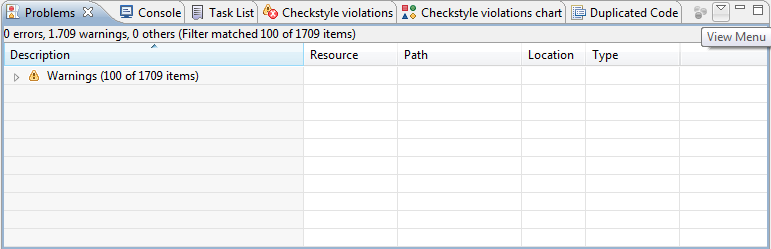
\includegraphics[width=1\textwidth]{pics/checkstyle1}
\end{center}
}
\frame{
\frametitle{Eclipse - mehr Fehler anzeigen}
\begin{center}
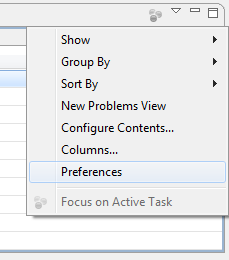
\includegraphics[width=0.5\textwidth]{pics/checkstyle2}
\end{center}
}
\frame{
\frametitle{Eclipse - mehr Fehler anzeigen}
\begin{center}
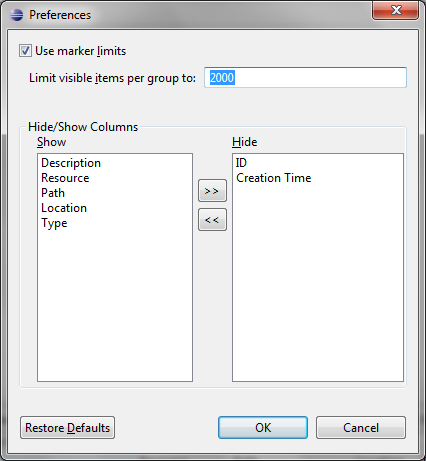
\includegraphics[width=0.5\textwidth]{pics/checkstyle3}
\end{center}
}

\subsection{Lastenheft}

\frame{
\frametitle{Lastenheft}
\begin{itemize}
\item enthält die Hauptanforderungen an das Produkt (user requirements)
\item formuliert mit natürlicher Sprache, evtl. Diagramme
\item dient der Kommunikation mit dem Kunden und der Projektplanung
\end{itemize}
}

\subsection{Klassendiagramm}
\frame{
\frametitle{Klassendiagramm: Erläuterung am Beispiel}
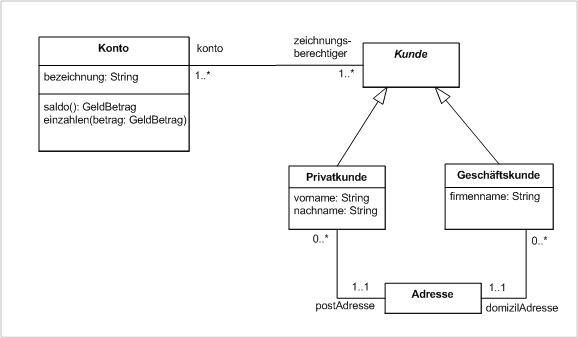
\includegraphics[scale=0.5]{pics/Klassendiagramm-1.png}
}

\frame {
\frametitle{Klassendiagramm Aufgabe}
\begin{block} {Szenario}  
In einer Formel 1-Saison gibt es 12 Teams. Die Saison hat 19 Rennen und an jedem Rennen nehmen
die Teams mit jeweils 2 Fahrzeugen teil. Während der Saison können Teams ausscheiden und von
nachrückenden Teams ersetzt werden. Es kann aber niemals in dieser Saison weniger als eins oder
mehr als 12 Teams geben. Zu den öffentlichen Eigenschaften eines Fahrzeugs gehört der Team-
Name, der Name des Chassis, die Motorbezeichnung sowie Startnummer und der Fahrer. Die Startnummer
ist eindeutig. Die geheimen Eigenschaften eines Fahrzeugs sind die Größe des Tanks und
die Dicke der Bodenplatte. In dieser Saison gibt es verschiedene Motoren, die von den zwölf Teams
in ihren beiden Fahrzeugen verbaut sind.
\end{block}

Verwenden Sie die aus der Vorlesung bekannten Vorgehensweisen zur Objektmodellierung und erstellen Sie
ein Klassendiagramm. Modellieren Sie dabei Klassen, Attribute, Assoziationen und Multiplizitäten.

}

\frame{
\frametitle{Musterlösung}
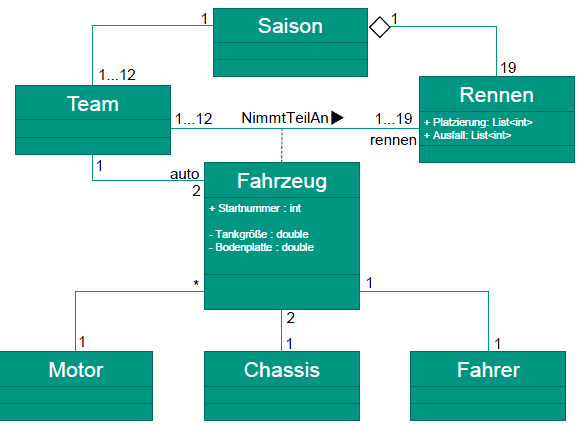
\includegraphics[scale=0.5]{pics/Klassendiagramm.png}

}

\subsection{Aktivitätsdiagramm}

\frame{
\frametitle {Aktivitätsdiagramm Allgemein} 
\begin{itemize}
	\item Ein Aktivitätsdiagramm beschreibt einen Ablauf
	\item Besteht aus \textbf{Aktions-, Objekt-} und \textbf{Kontrollflussknoten} sowie \textbf{Objekt-} und 											\textbf{Kontrollflüssen}
	\item Elemente eines Aktivitätsdiagramms
	\begin{itemize}
		\item Aktionen
		\item Knoten (Startknoten, Endknoten, Ablaufende)
		\item Entscheidungen (durch Raute dargestellt)
		\item Zusammenführung
		\item Aufteilung des Kontrollflusses
		\item Synchronisation
	\end{itemize}
\end{itemize}
}

\frame {
\frametitle{Beispiel}
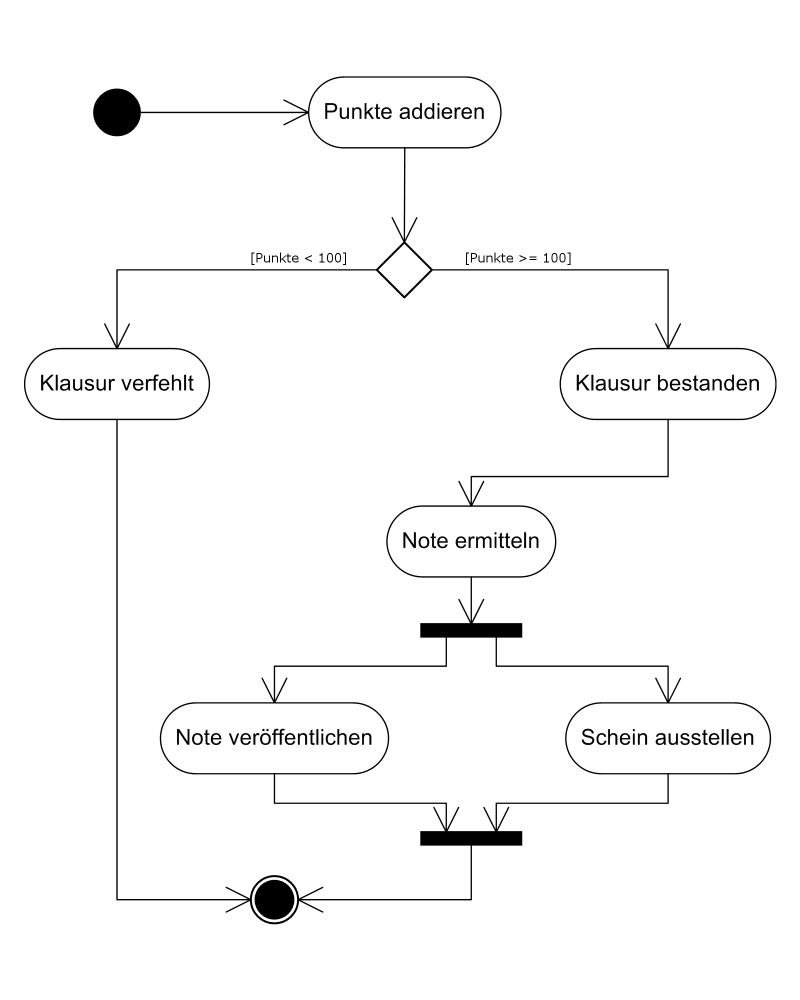
\includegraphics[scale=0.22]{pics/beispiel.png}
}
\frame{
\frametitle{Aufgabe Aktivitätsdiagramm (9P)}
\small {
Nach dem Start beginnt die erste Runde. 
In dieser und in jeder folgenden Runde
kann sich der Fahrer entscheiden, ob er an
die Box kommen oder die Runde fahren
möchte. Nach der letzten Runde ist das
Rennen unmittelbar beendet. Der Boxenstopp
beginnt damit, dass der Fahrer den
Rennwagen auf die in der Boxengasse
erlaubte Höchstgeschwindigkeit abbremst.
Anschließend parkt er seinen Rennwagen in der Box. Sobald der Rennwagen steht, wird
er von einem Mitarbeiter der Boxencrew angehoben. Danach werden von vier weiteren
Mitarbeitern der Boxencrew gleichzeitig die Räder gewechselt, wobei sich jeder Mitarbeiter
um jeweils ein Rad kümmert. Neben dem Radwechsel wird der Rennwagen frisch
betankt, was ebenfalls ein dedizierter Mitarbeiter erledigt. Sobald alle vier Räder gewechselt
sind, kann der Rennwagen abgelassen werden. Der Fahrer fährt los, sobald der
Rennwagen abgelassen und der Tankvorgang beendet wurde. Sobald der Fahrer das
Ende der Boxengasse erreicht hat, beschleunigt er den Rennwagen auf Renntempo und
fährt die Runde zu Ende. Anschließend geht der Fahrer auf die nächste Runde oder das Rennen ist
beendet.
}
}

\frame{
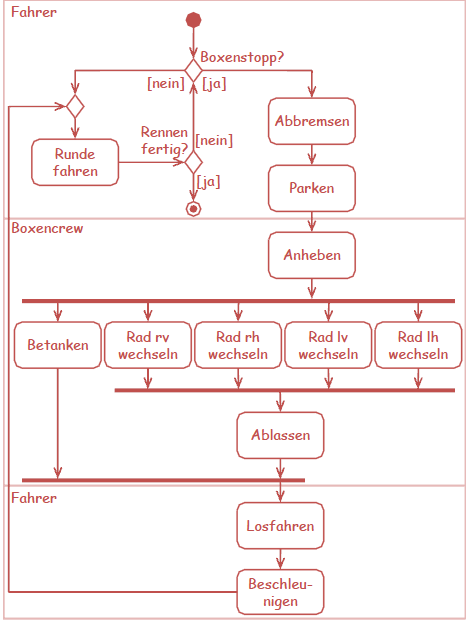
\includegraphics[scale=0.5]{pics/diagramm.png}
}
\subsection{Pflichtenheft}

\frame{
\frametitle{Pflichtenheft}
\begin{itemize}
\item Das Pflichtenheft ist eine Verfeinerung des Lastenheftes\pause
\item Das Pflichtenheft beschreibt nicht, wie, sondern nur \textbf{was} zu implementieren ist. \pause
\\ $\Rightarrow$ es werden weder Algorithmen noch Datenstrukturen festgelegt \pause
\item das Pflichtenheft definiert das Projekt so vollständig und exakt, \\
dass Entwickler das System implementieren können, \\
ohne nachfragen oder raten zu müssen, \textbf{was} zu implementieren ist.
\end{itemize}
}

%%%%%%%%%%%%%%%%%% kommt erst noch?
%\frame{
%\frametitle{Pflichtenheft}
%\begin{block}{Gliederungsschema Pflichtenheft}
%\begin{itemize}
%\item\dots
%\end{itemize}
%\end{block}
%}



\section{Ende}

\frame{
\frametitle{Tipps zum nächsten Übungsblatt}

\begin{block}{Aufgabe 1 - Klassendiagramm}
\begin{itemize}
\item denkt an Attribute, Multiplizitäten, Restriktionen, Assoziationsnamen sowie Rollen \pause
\item merkt euch den Unterschied zwischen Komposition und Aggregation!
\end{itemize}
\end{block}

\begin{block}{Aufgabe 2 - Aktivitätsdiagramm}
\begin{itemize} \pause
\item ihr dürft die Aufgabe auf zwei Diagramme verteilen \pause
%\item Bla bla
\end{itemize}
\end{block}

\begin{block}{Aufgabe 3 - Programmieren}
\begin{itemize}
\item args4j kann euch sehr viel Arbeit ersparen, versucht die Bedienung anhand von Configuration.java zu verstehen \pause
\item achtet darauf ob ihr Ganzzahldivision verwendet: \\ \pause
\texttt{int o; \dots; int p = (o + 128 ) / 256 * 255 \\
		// liefert hier 0 oder 255: wieso?}
\end{itemize}
\end{block}


}


\frame{
\frametitle{Bis zum nächsten Mal}
\begin{center}
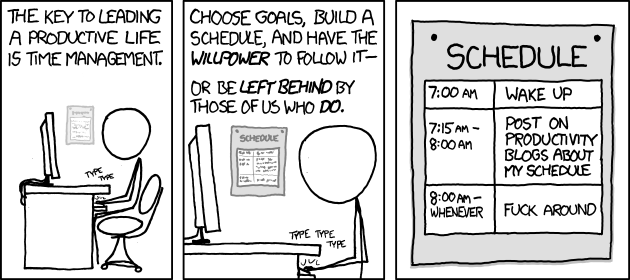
\includegraphics[width=1\textwidth]{pics/time_management}
\end{center}

}


\end{document}
